After completion of the design and construction of the tachometer hardware and software, tests were conducted to ensure all specifications of the contract were met. These tests included measuring hardware design limits and confirming the device operates as intended.


\subsection{Ignition Signal Simulation}
Effectively designing a conditioner for the ignition signal required a running engine, however this was not practical. An ignition simulator was built that produced an output similar to that in Figure~\ref{fig:boat_noise}, and was used to design the ignition signal conditioner. Figure~\ref{fig:sim_raw} shows the output from the ignition simulator.

\begin{figure}[H]
    \centering
    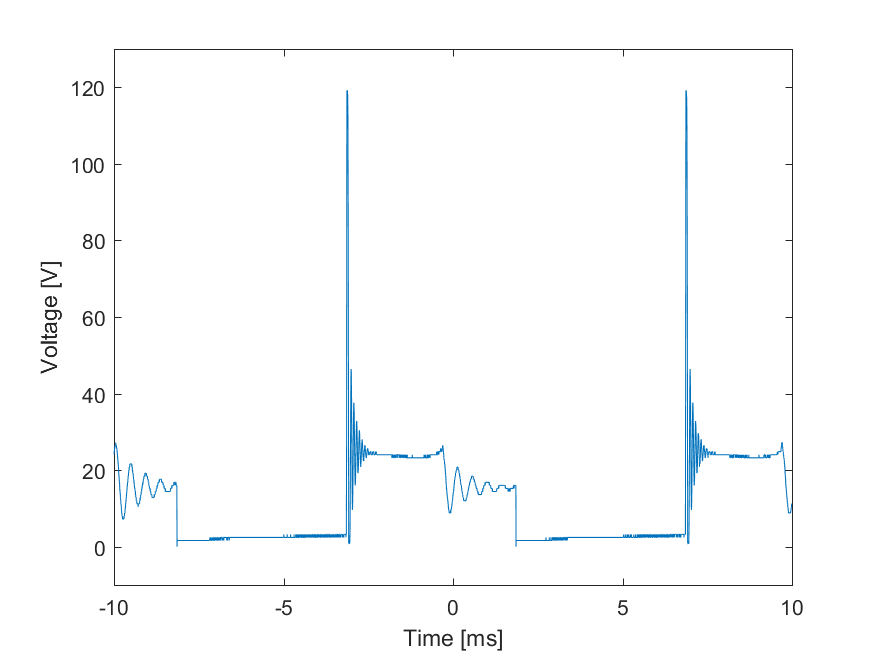
\includegraphics[width=\textwidth]{sim_raw}
    \caption{Engine ignition system}
    \label{fig:sim_raw}
\end{figure}

The ignition simulator works much the same way as the actual ignition system on a gasoline engine. It uses an ignition coil, condenser, and spark plug from a car engine. Instead of points, it has a transistor controlled by a function generator to simulate any desired engine RPM. As seen in the Figure above, the output from the simulator is very similar to that measured on the gasoline engine. The simulator allowed design and testing of the ignition signal generator to be performed in a lab without a running engine.


\subsection{Specifications}
With the ignition signal simulator, the tachometer's primary function could be tested. Using the signal generated by the simulated ignition as an input allowed the response of the gauge to be observed. The power supply, tachometer operation, and deliverability specifications are discussed in their own sections in further detail.

The engine sensor input operation was confirmed by simulating the engine sensors with a potentiometer circuit. A calibration routine is in place such that the tachometer can be calibrated to the sensors on the power boat. The detachable display is the method for displaying the sensor's outputs.

\subsubsection{Power Supply}
The power supply was required to have an output voltage within 5\% of the specified output and less than 100mV of ripple. With the power supply constructed, both of these specifications were measured. Shown below in Figure~\ref{fig:ps_dc} is the output of the power supply, measured with DC coupling on an oscilloscope.

\begin{figure}[H]
    \centering
    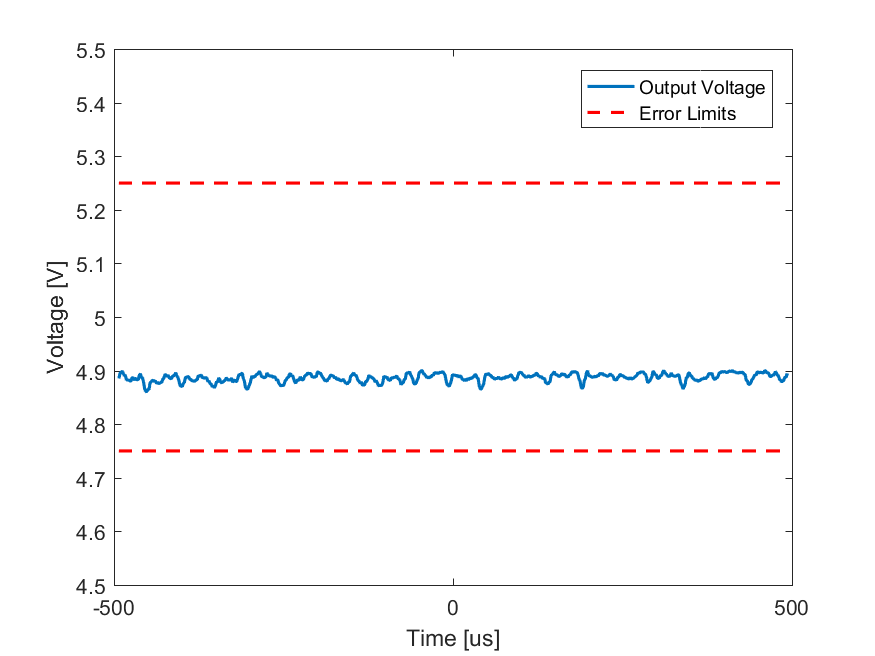
\includegraphics[width=\textwidth]{power_supply_dc}
    \caption{Power supply output, DC coupling}
    \label{fig:ps_dc}
\end{figure}

The output voltage was found to be well within the specified 5\% error region. By switching the oscilloscope to AC coupling, the output ripple was more easily measured. Shown below in Figure~\ref{fig:ps_ac} is the output ripple of the power supply.

\begin{figure}[H]
    \centering
    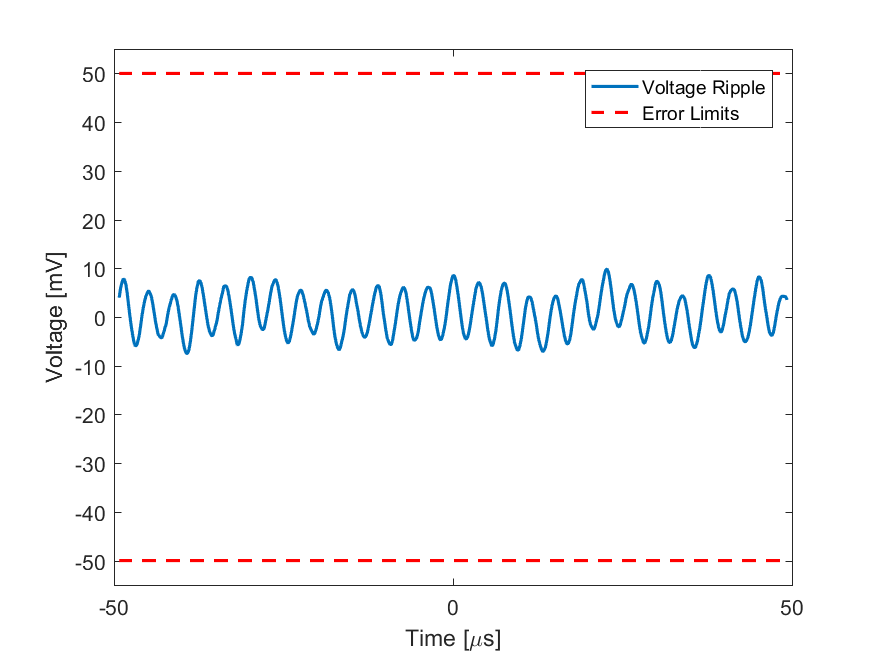
\includegraphics[width=\textwidth]{power_supply_ac}
    \caption{Power supply output, AC coupling}
    \label{fig:ps_ac}
\end{figure}

The ripple is around 20m$V_{PP}$, significantly lower than the specified 100m$V_{PP}$. Furthermore, the power supply PCB was laid out such that a total of five output capacitors could be populated, however only two were needed to achieve this result. If lower ripple was desired, more capacitors could be added to further improve the power supply's performance.

\subsubsection{Tachometer Operation}
Tachometer operation was verified in two separate ways: first with the ignition signal simulation, and second by connecting it to a car with a four cylinder engine. These tests showed that the tachometer and power supply were capable of operating with the presence of the ignition and other electrical system noise from the vehicle. The accuracy of the tachometer output was measured by comparing the gauge and LCD output values against known input values, results are shown in Figure~\ref{fig:rpm}.

\begin{figure}[H]
    \centering
    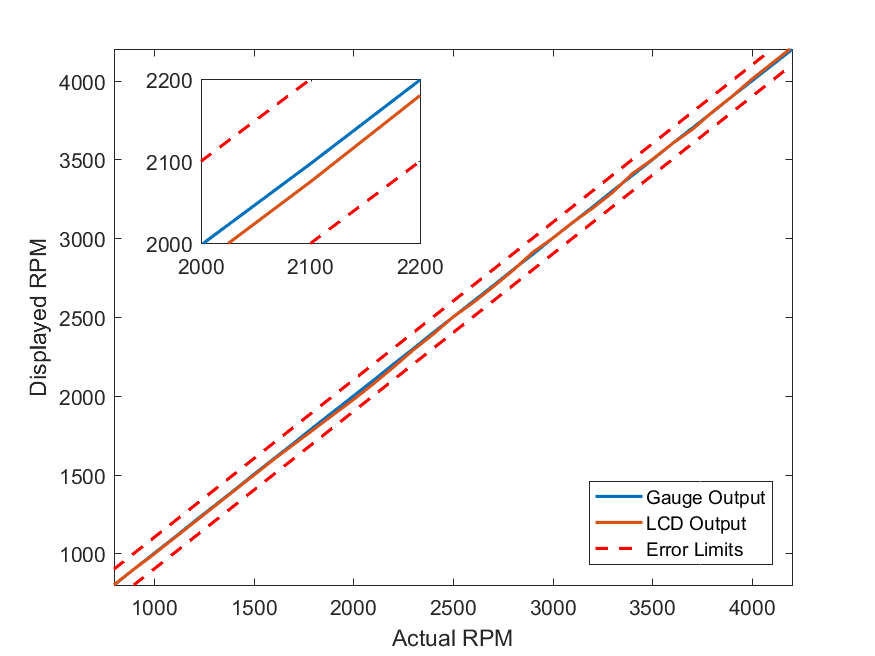
\includegraphics[width=\textwidth]{rpm}
    \caption{Gauge and LCD output accuracy}
    \label{fig:rpm}
\end{figure}

The plot shows both the LCD and gauge were within the $\pm$100 RPM error limits, with little variation between the two outputs. Furthermore, the tests revealed that under typical operation, the gauge and LCD outputs are within 10 RPM of the measured value.

\subsubsection{Deliverability}
As specified, the tachometer is deliverable to the customer with a box and secure mounting hardware protect the PCB and internal components. Proper mounting, connectors, and cable relief ensure long life of the tachometer. 

Additionally, Appendix~\ref{app:user} includes documentation on the installation and use of the tachometer. The documentation is useful for the owner of the product or service technician to diagnose problems or perform a new installation.

Since the tachometer is designed to work with any engine, not just that of the 1988 Celebrity Champion, it features user calibration. Since all tachometer gauges and all engine sensors are slightly different, the tachometer must be calibrated on a per-installation basis. Calibration is done via a serial connection and features a simple, intuitive interface for calibrating the range of the tachometer gauge and the range of the analog engine sensors. As discussed in a previous section, the tachometer was tested for proper operation in a car. This proves that the tachometer can be calibrated to work in various installation environments.

Additionally, while the contract specifies that a DC-DC converter is to be built and there are to be other engine sensor inputs, the customer is mainly interested in reliable tachometer operation. Since off-the-shelf DC-DC components are often more reliable than custom power supplies, the tachometer is designed such that a linear (or switching linear replacement) could replace the power supply designed to meet contract specifications. The sensor inputs are also constructed on a different PCB, such that they do not take up additional space, or draw additional power if the customer chooses not to use them.

